%file included in thesis.tex

\chapter{Implementation}
In this chapter implementation specific issues are treated. Figure
\ref{chap6:fig-implementation} shows the three-layer implementation of the project.
\begin{figure}[htbp]
    \centering
    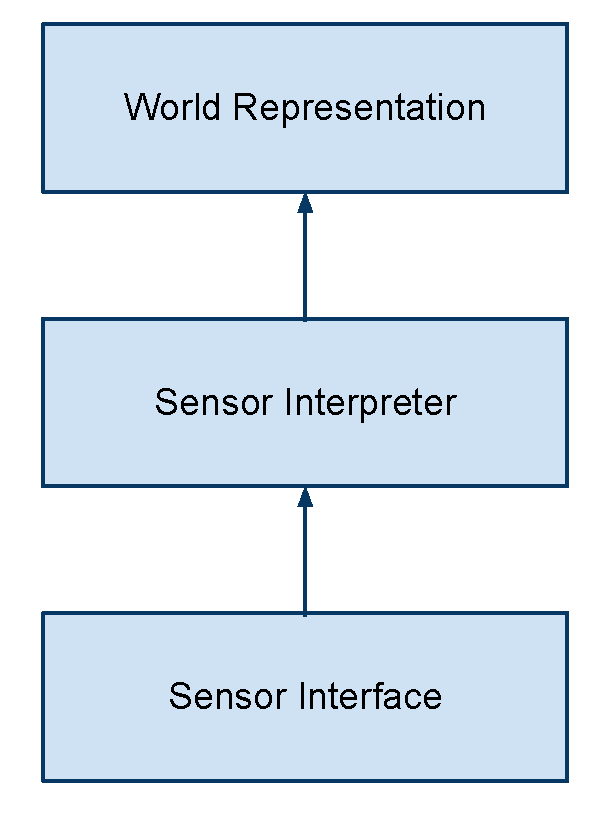
\includegraphics[width=0.4\textwidth]{pics/implementation}
    \caption{Three-layer implementation}
    \label{chap6:fig-implementation}
\end{figure}
The \emph{low-level} layer reads and converts the raw sensor data into common data which can be
interpreted by the \emph{middle} layer. This layer handles all the ''washing`` of the
sensor data, and applies the reasoning and tries to recognize the environment. The third
and last layer is the \emph{world} layer which handles the global data, where the robot is
and where it should move next. 

The project is implemented in both \emph{C/C++} and Matlab. The sensor layer are
implemented in \emph{C/C++} while the other layers are implemented in Object-Oriented
Matlab. 

\section{Low-level Interfaces}
The low-level interfaces from the sensors are implemented in \emph{C/C++} and uses the
supplied sensor APIs. The SwissRanger 3000 API were used directly in Matlab. The Hokuyo
API was a little more tricky to use. A Matlab interface function were implemented to get
the sensor data directly into Matlab.

\subsection{Stereo Camera Implementation}
For the stereo camera, a program was written using the \emph{OpenCV} library. A open
source computer vision library, initially developed by Intel. This library have many
excellent and optimized functions for grabbing images, camera calibration, image rectification
and stereo matching. This produced a disparity map, which again where reprojected into 3D
by the \emph{cvReprojectTo3D()}-function. This coordinate images where saved to disk and
read into Matlab for further processing. 

\begin{algorithm}
\caption{The Stereo Capture Procedure}
\label{chap6:alg-stereomatch}
    \begin{algorithmic}
    \STATE \textbf{begin}
    \STATE Connect to Cameras
    \FOR{no of images $<$ 20}
        \STATE Capture images of Checkerboard and find corners
    \ENDFOR
    \STATE Calculate the distortion parameters using Healy's Method.
    \WHILE{Not Quitting}
        \STATE Capture images
        \STATE Rectify Images
        \STATE Stereo matching using Block Matching 
        \STATE Reproject disparity map to 3DImage
        \STATE Dump 3D Coordinates to Disk
    \ENDWHILE
    \STATE \textbf{end}
    \end{algorithmic}
\end{algorithm}
This program calibrates the cameras, rectifies the images, finds stereo correspondences
and reprojects them to 3D coordinates.


\section{Mid-level Implantations}
The middle layers goal is to process and interpret the sensor data to best ability. This
layer is in charge of doing the reasoning, and draw out important information form the
sensor data. The main task is to find lines in the 2D sensor data, and cylinder shapes in
the 3D data. 

This functionality are implemented in a Matlab class called the \emph{SensorInterpreter}.


\subsection{Analysis of 3D Sensor Data}
The 3D data are first filtered with regard to corresponding the intensity image. Pixels
with intensities larger or lower than a threshold value will be filtered away and set to
zero. 

After this the coordinates are sorted on ascending depth value, and all trivial points,
i.e. zero points are taken out of the coordinate list. The new list with coordinates
including only interesting points will be divided into 10 equally spaced bins in the depth
direction. Each of this bins are sent to the surface fit algorithm which is a
\emph{Least-Squares Guass-Newton steepest decent}-algorithm. 

\subsubsection{Surface Fit Algorithm}
The algorithm which is used are the \emph{EUROMETROS}\cite{eurometros} Matlab library developed by
\emph{National Physics Laboratory(NPL)} in the United Kingdom. The algorithm provides the
estimated radii, and directions of the data sets. Also the distance of the data set to the
estimated cylinders are output, which is a measurement on how good the cylinder fit is. 

\paragraph{Issues}
The algorithm is sensitive to edge data. This can be controlled with limiting the interval
in the z-direction of which the cylinder is fitted to the data.*************FIX*******


\section{High-level Implementations}

\subsection{World Representation}
The world representation are implemented as objects in Matlab. Each node in the world
representation described in Chapter \ref{chap5} are implemented as a class in Matlab. 
\begin{figure}[htbp]
    \centering
    %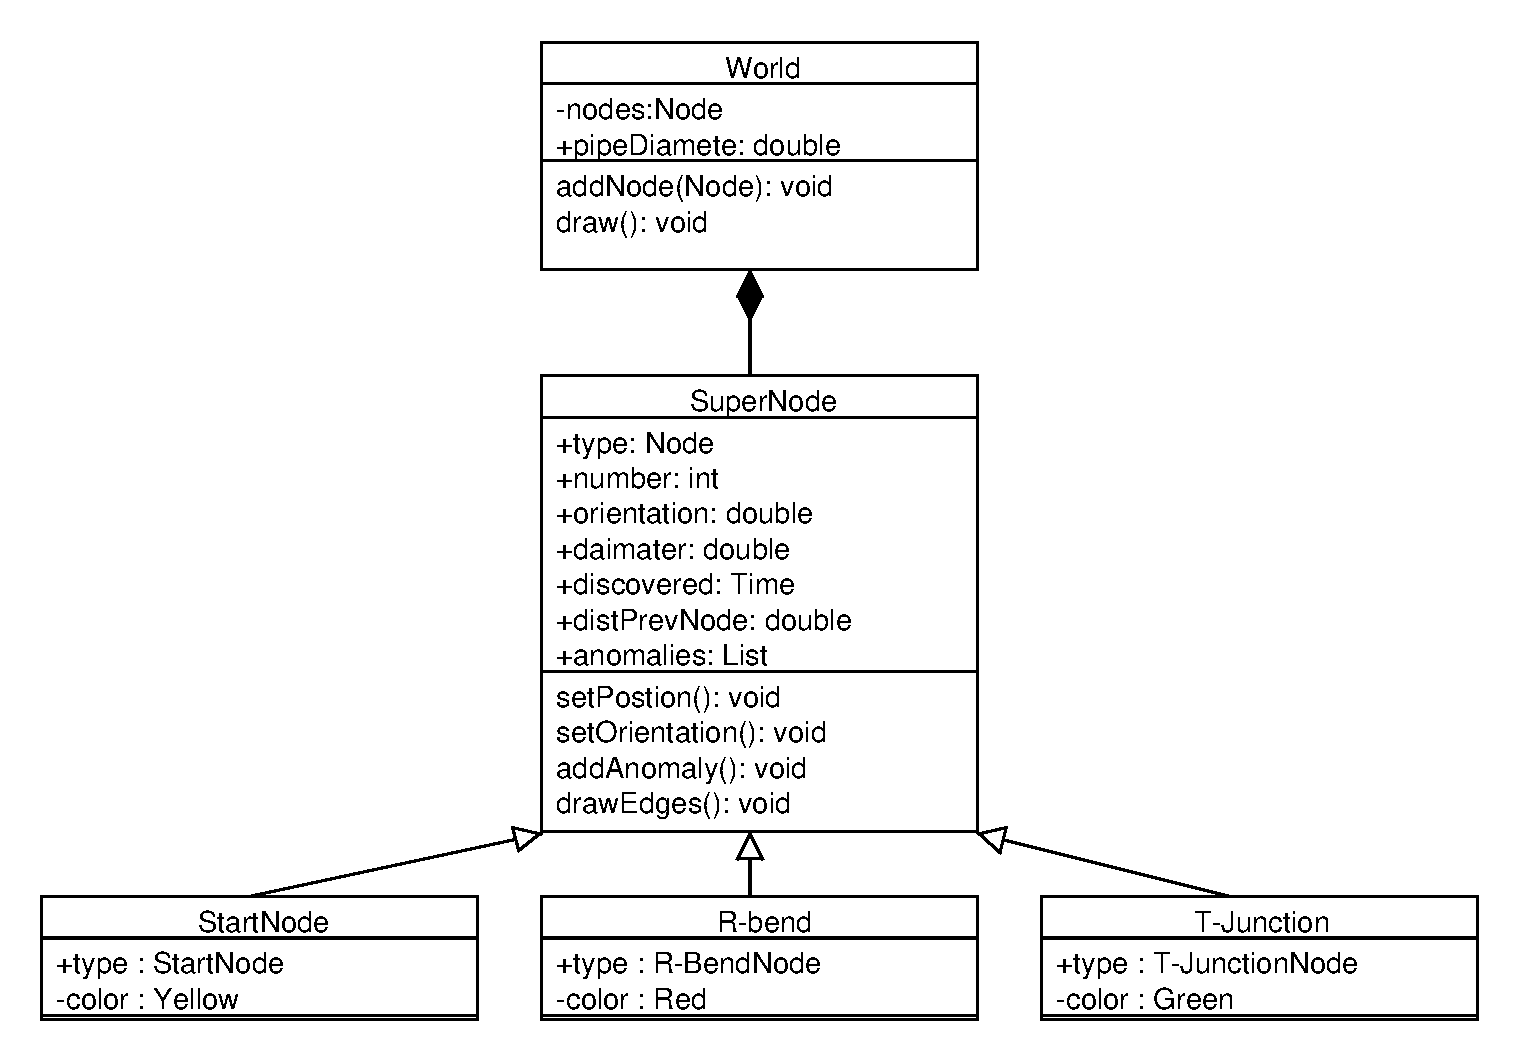
\includegraphics[width=0.6\textwidth]{pics/world-uml}
    \caption{UML of the world representation}
    \label{chap6:fig-world-uml}
\end{figure}

As seen from Figure \ref{chap6:fig-world-uml} the implementation are based on a
\emph{world} class which contains the á priori map of the world and the node network
together with some useful parameters. The nodes of the representation are also different
classes which inherits from a super node. 





